\documentclass[tikz,border=10pt]{standalone}

\usepackage{xcolor}
\usetikzlibrary{arrows.meta, positioning}

\definecolor{paperGreen}{RGB}{34,125,92}
\definecolor{paperGold}{RGB}{176,125,33}
\definecolor{paperSoft}{RGB}{246,248,250}
\definecolor{paperLine}{RGB}{80,92,110}

\begin{document}
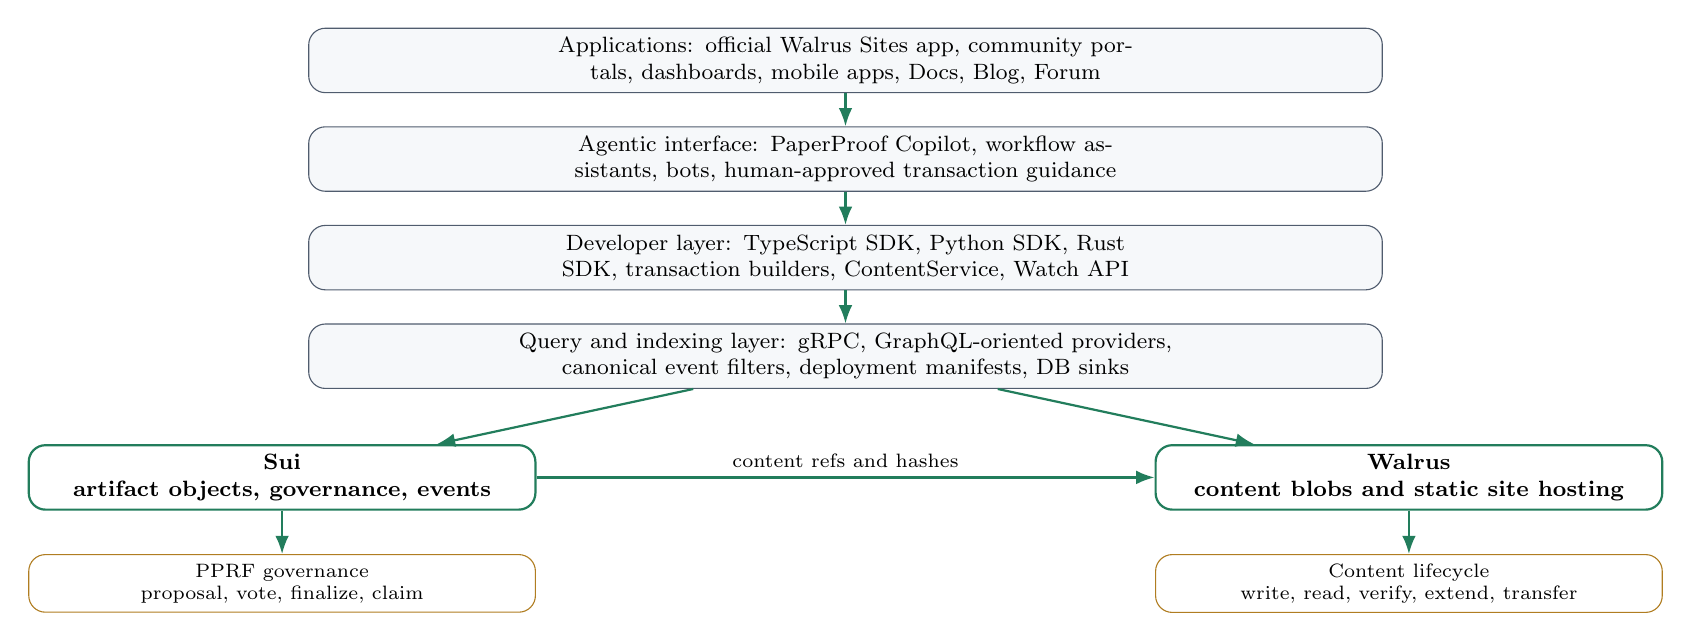
\begin{tikzpicture}[
    layer/.style={draw=paperLine, rounded corners=6pt, fill=paperSoft, minimum height=0.75cm, align=center, font=\footnotesize, text width=13.4cm},
    base/.style={draw=paperGreen, thick, rounded corners=6pt, fill=white, minimum height=0.78cm, align=center, font=\footnotesize\bfseries, text width=6.2cm},
    side/.style={draw=paperGold, rounded corners=6pt, fill=white, minimum height=0.7cm, align=center, font=\scriptsize, text width=6.2cm},
    arrow/.style={-Latex, thick, draw=paperGreen},
    node distance=0.42cm
]
    \node[layer] (apps) {Applications: official Walrus Sites app, community portals, dashboards, mobile apps, Docs, Blog, Forum};
    \node[layer, below=of apps] (agents) {Agentic interface: PaperProof Copilot, workflow assistants, bots, human-approved transaction guidance};
    \node[layer, below=of agents] (sdk) {Developer layer: TypeScript SDK, Python SDK, Rust SDK, transaction builders, ContentService, Watch API};
    \node[layer, below=of sdk] (query) {Query and indexing layer: gRPC, GraphQL-oriented providers, canonical event filters, deployment manifests, DB sinks};
    \node[base, below left=0.7cm and -2.9cm of query] (sui) {Sui\\artifact objects, governance, events};
    \node[base, below right=0.7cm and -2.9cm of query] (walrus) {Walrus\\content blobs and static site hosting};
    \node[side, below=0.55cm of sui] (gov) {PPRF governance\\proposal, vote, finalize, claim};
    \node[side, below=0.55cm of walrus] (content) {Content lifecycle\\write, read, verify, extend, transfer};

    \draw[arrow] (apps) -- (agents);
    \draw[arrow] (agents) -- (sdk);
    \draw[arrow] (sdk) -- (query);
    \draw[arrow] (query) -- (sui);
    \draw[arrow] (query) -- (walrus);
    \draw[arrow] (sui) -- (gov);
    \draw[arrow] (walrus) -- (content);
    \draw[arrow] (sui) -- node[above, font=\scriptsize] {content refs and hashes} (walrus);
\end{tikzpicture}
\end{document}
